\subsection{Invarient stress: Flow and storage in a compressible medium}

It is also possible, and sometimes useful, to test two-phase storage and pressure dissipation in a deformable media at invarient stress. This test guarantees accurate implementation of fluid storage within the mass matrix (time derivative term) of the fluid mass balance PDE. 

\subsubsection*{Definition}
We utilize the same problem as above, but now no stress is applied and no mechanical equilibrium performed. The analytical solution may be derived from the Carslaw and Jaeger \cite{Carslaw:59} solution for heat dissipation within a solid slab,

\begin{equation}
\bar{p}\left( z,t \right)=\frac{4{{p}_{0}}}{\pi }\sum\limits_{m=0}^{\infty }{\left\{ \frac{1}{2m+1}\sin \left[ z\left( \frac{\left( 2m+1 \right)\pi }{2L} \right) \right]\exp \left[ -ct{{\left( \frac{\left( 2m+1 \right)\pi }{2L} \right)}^{2}} \right] \right\}},
\end{equation}

where $\bar{p}_0$ is initial mean pressure within the column.

\begin{figure}[!b]
\begin{center}
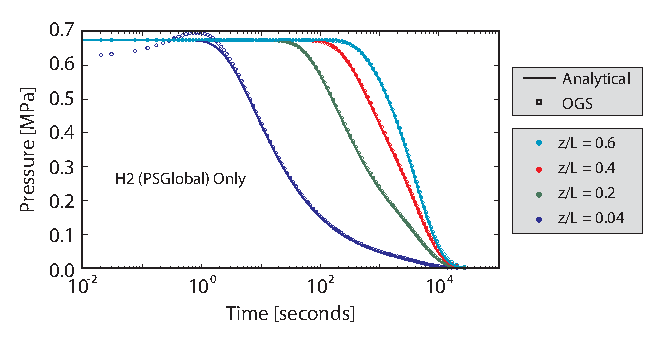
\includegraphics[width=0.7\textwidth]{chapter_14/figures/fig_14_3_23}
\end{center}
\caption{Two-phase flow with mechanical storage.}
\label{terz:h2}
\end{figure}

\subsubsection*{Results}
Results are shown in Fig. \ref{terz:h2}. We note that with an appropriate mixing rule for storage in the two phase formulation, the result is ideal.  Very small values of time and $z$ can produce inaccuracies; however, this will always be the case, barring a very small mesh discretization.